\documentclass{ltjsarticle}
\usepackage{docmute} 
\usepackage{myStyle} 

\begin{document}

\chapter{要因計画と平均値差の検定}
\label{chapter21}
ここまでは主に，平均値の比較に確率的判断の手続きを加えた仮説検定の話をしてきました。
ここでは前期の最後に学んだ，線形モデルから要因計画へと進んだ話に，検定の話を統合します。線形モデルに確率的判断の手続きを加えたものが，分散分析と呼ばれる独自の体系になります。ここでは線形モデルの一環であることを意識しつつ，質的説明変数によって水準同士の対比較になることによる分析の手順について理解することを目的とします。水準が多くなった場合の対比較には，検定の多重性の問題が影響してくるため，問題を回避するために多重比較と言う考え方も導入する必要があります。

\section{平均値の比較とモデル比較}
前期の話の流れを思い出すと，わからないことをモデルで考え(第\ref{chapter5},\ref{chapter6},\ref{chapter7}章)，関係性を線形モデルで表現し(第\ref{chapter8},\ref{chapter9}章)，その特例(説明変数が離散的)としての実験計画法(第\ref{chapter12},\ref{chapter13},\ref{chapter14}章)，という流れでした。

後期に入ってから，確率の使い方が母集団を対象にしたものに変わりました。これまでは誤差が正規分布するから，という理由で確率が導入されていましたが，様々な誤差に影響された誤差まみれの数字は，正規分布するという正規分布の別の側面からアプローチしてきたのです。また，母集団と標本という区別をおくことで，母集団の分布についての仮定から，標本統計量の分布が考えられ，それを使って母数を推測するという方法を取りました。母数を推測するだけでなく，実践的な判断をする帰無仮説検定という手続きについても，解説してきました。

\begin{wrapfigure}{r}{8cm}
    \centering
    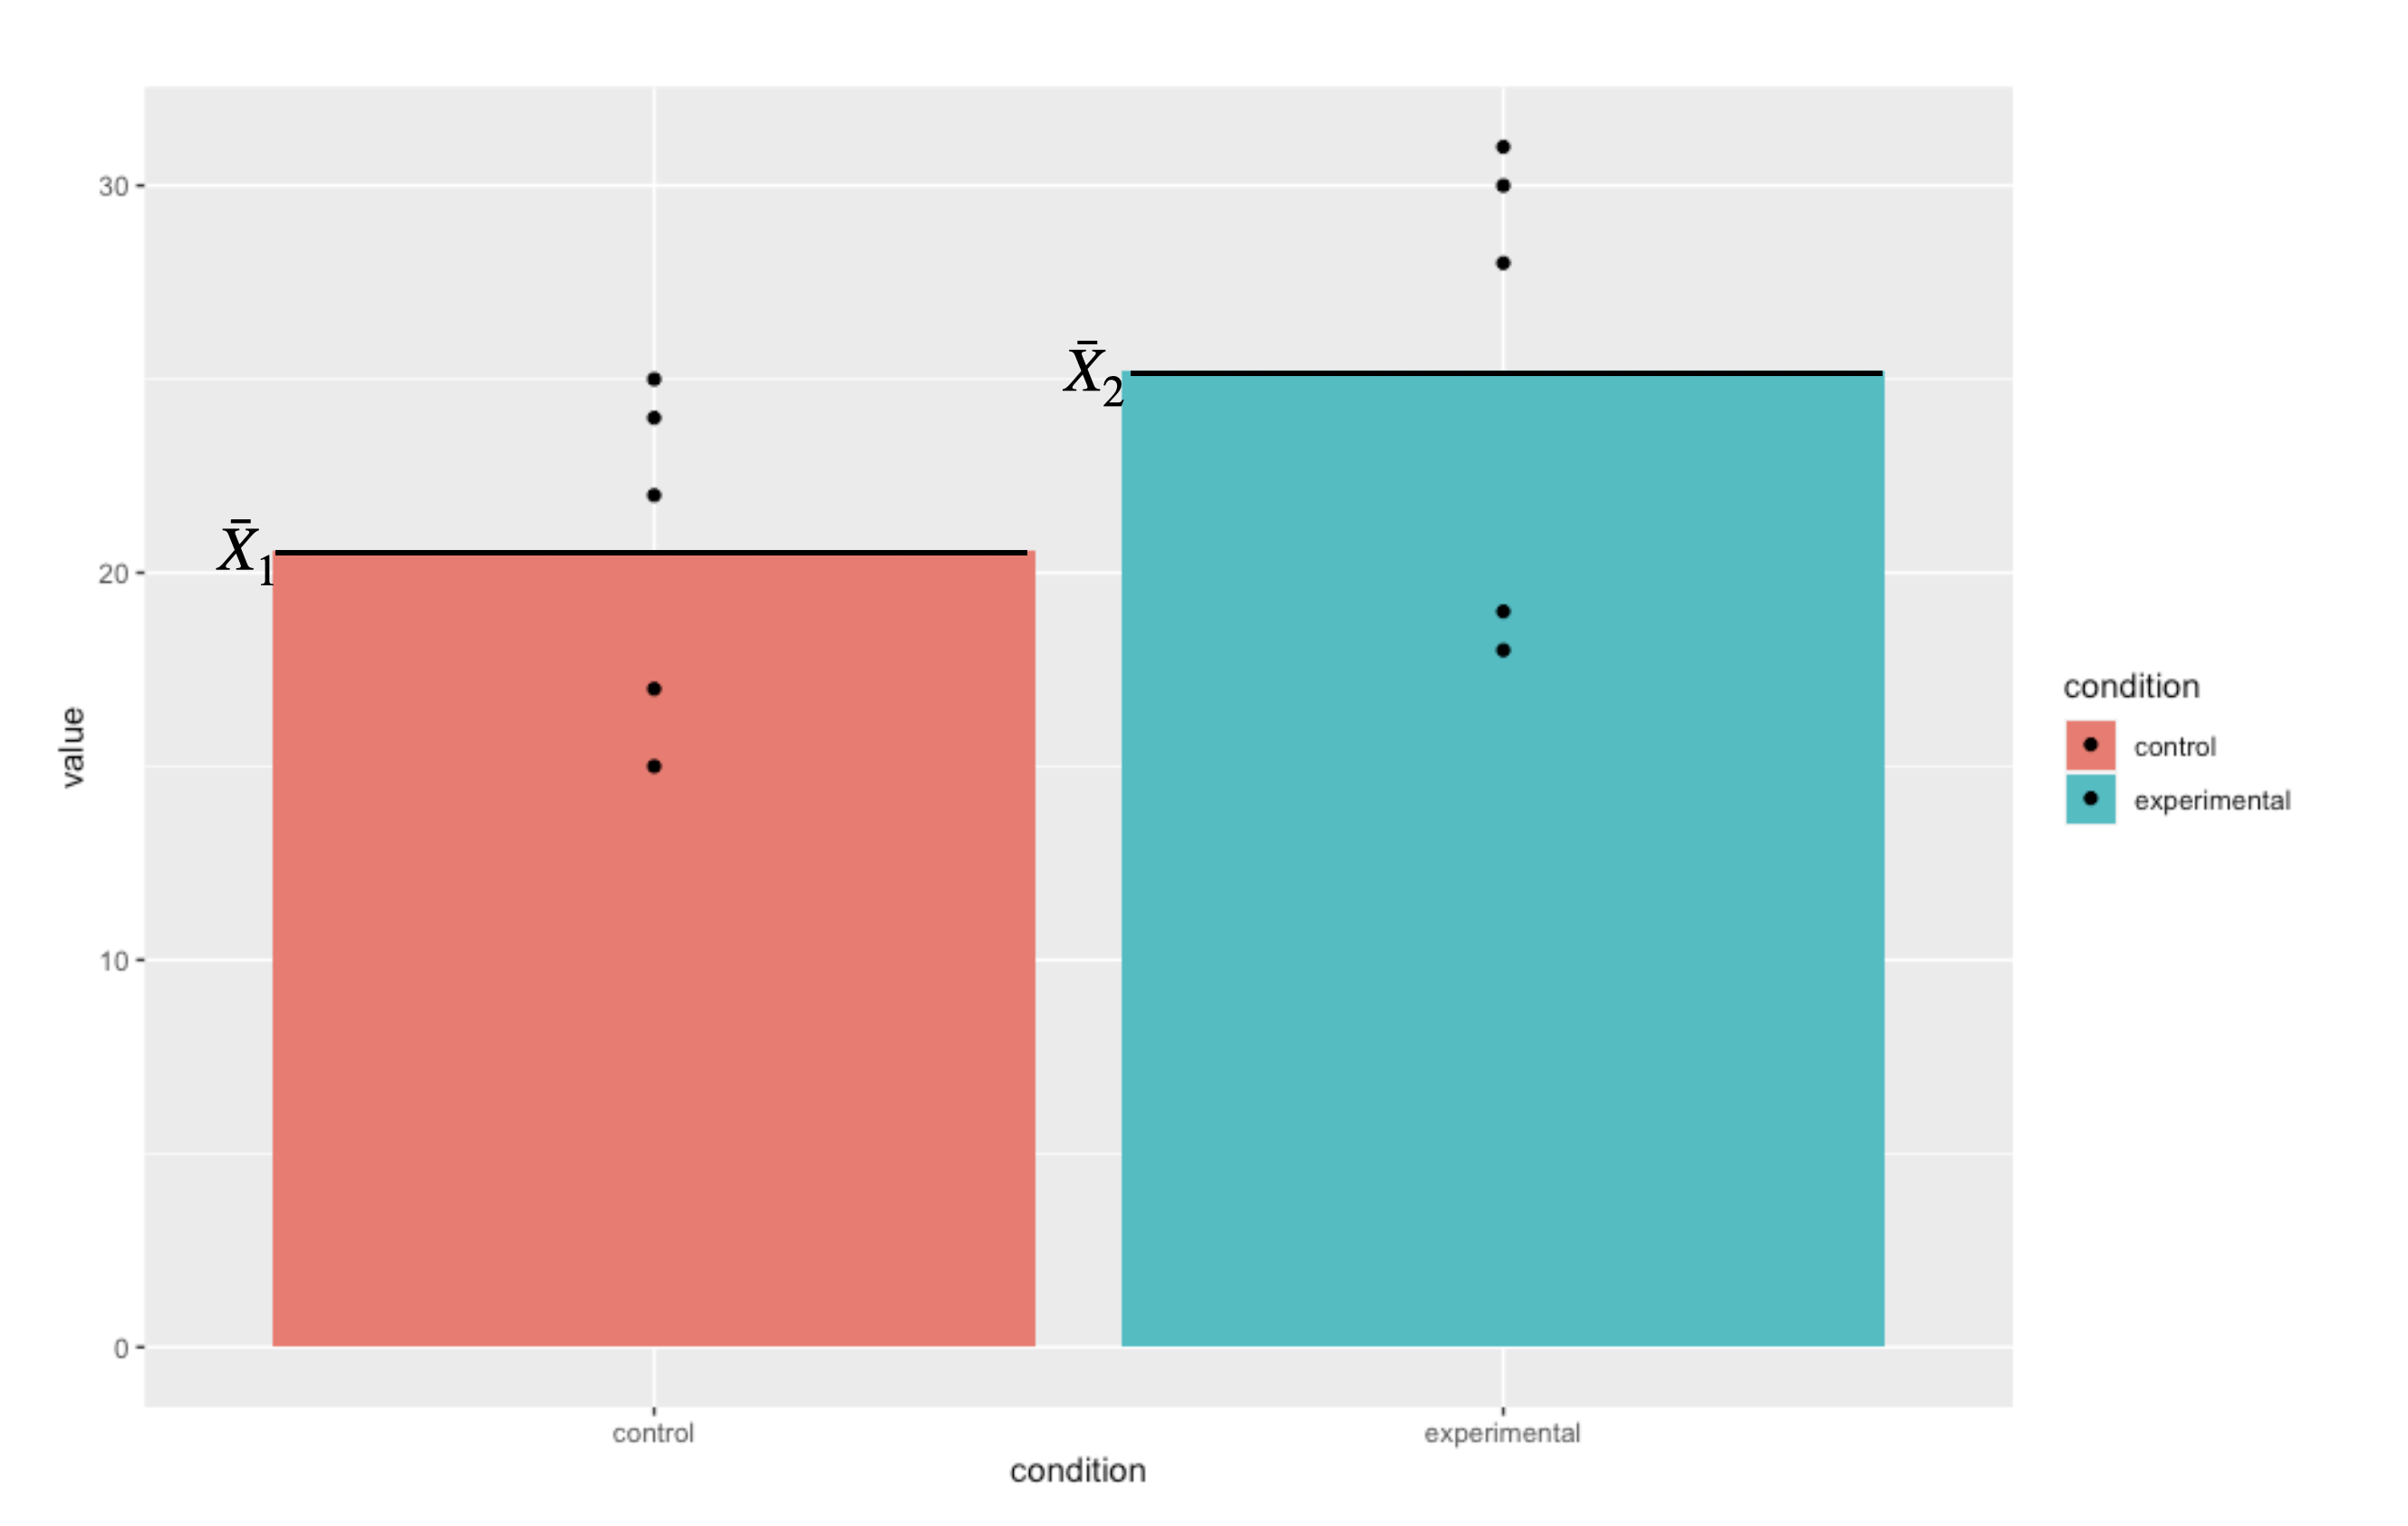
\includegraphics[keepaspectratio,width=8cm]{images/text21/slide21_01.png}
    \caption{2つの群の平均値のプロット。黒い点は各群のそれぞれの観測値}
    \label{fig::21_01}
\end{wrapfigure}

さて，最初に帰無仮説検定の話をしたときに，これはモデル比較だと言いました。帰無仮説というモデル，対立仮説というモデルを比較して，どちらに軍配を上げるかという勝負判定をする，これが帰無仮説検定だと。
ここでの「モデル」という言葉は，例えば帰無仮説は$\mu_1 - \mu_2 =0$とおく，といった表現がなされますから，前期の(線形)モデルという表現と異なるイメージを持ったかもしれません。しかしこれもモデル，しかも線形のモデルなのです。今からこの「帰無仮説検定」と「線形モデル」を概念的に統合することを説明してきます。

そのための例として，次のようなデータを用意しました(図\ref{fig::21_01})。これは対応のない，2つの群(仮に実験群と統制群とします)の平均値をプロットしたものです。ここで示されている平均値は標本平均ですから，そこに差があるのは見た通りです。ちなみに黒い点は各群における個体1つ1つの観測値です。

\subsection{平均値差の検定として考える}
まずは最近ずっと取り組んでいる，この標本平均から母平均を推測することを考えましょう。私たちは目の前のデータのこと「だけ」について考えているのではなく，議論を一般化したいのですから。母集団に正規分布を仮定すると，標本標準偏差や$t$分布を使って母平均を推測できるのでしたね。

さて，ここで帰無仮説検定の，母平均に差がないと言うのはどういう状況でしょうか。$\mu_1 - \mu_2 =0$ というのはつまり，$\mu_1 = \mu_2$ということと同じですから，同じ平均値を持つ正規分布からデータが得られたと仮定した，と言うことになります(図\ref{fig::21_04})\footnote{特に$t$検定においては標準偏差も同じと仮定しますから，同一の正規分布になります}。
\begin{figure}[ht]
    \centering
    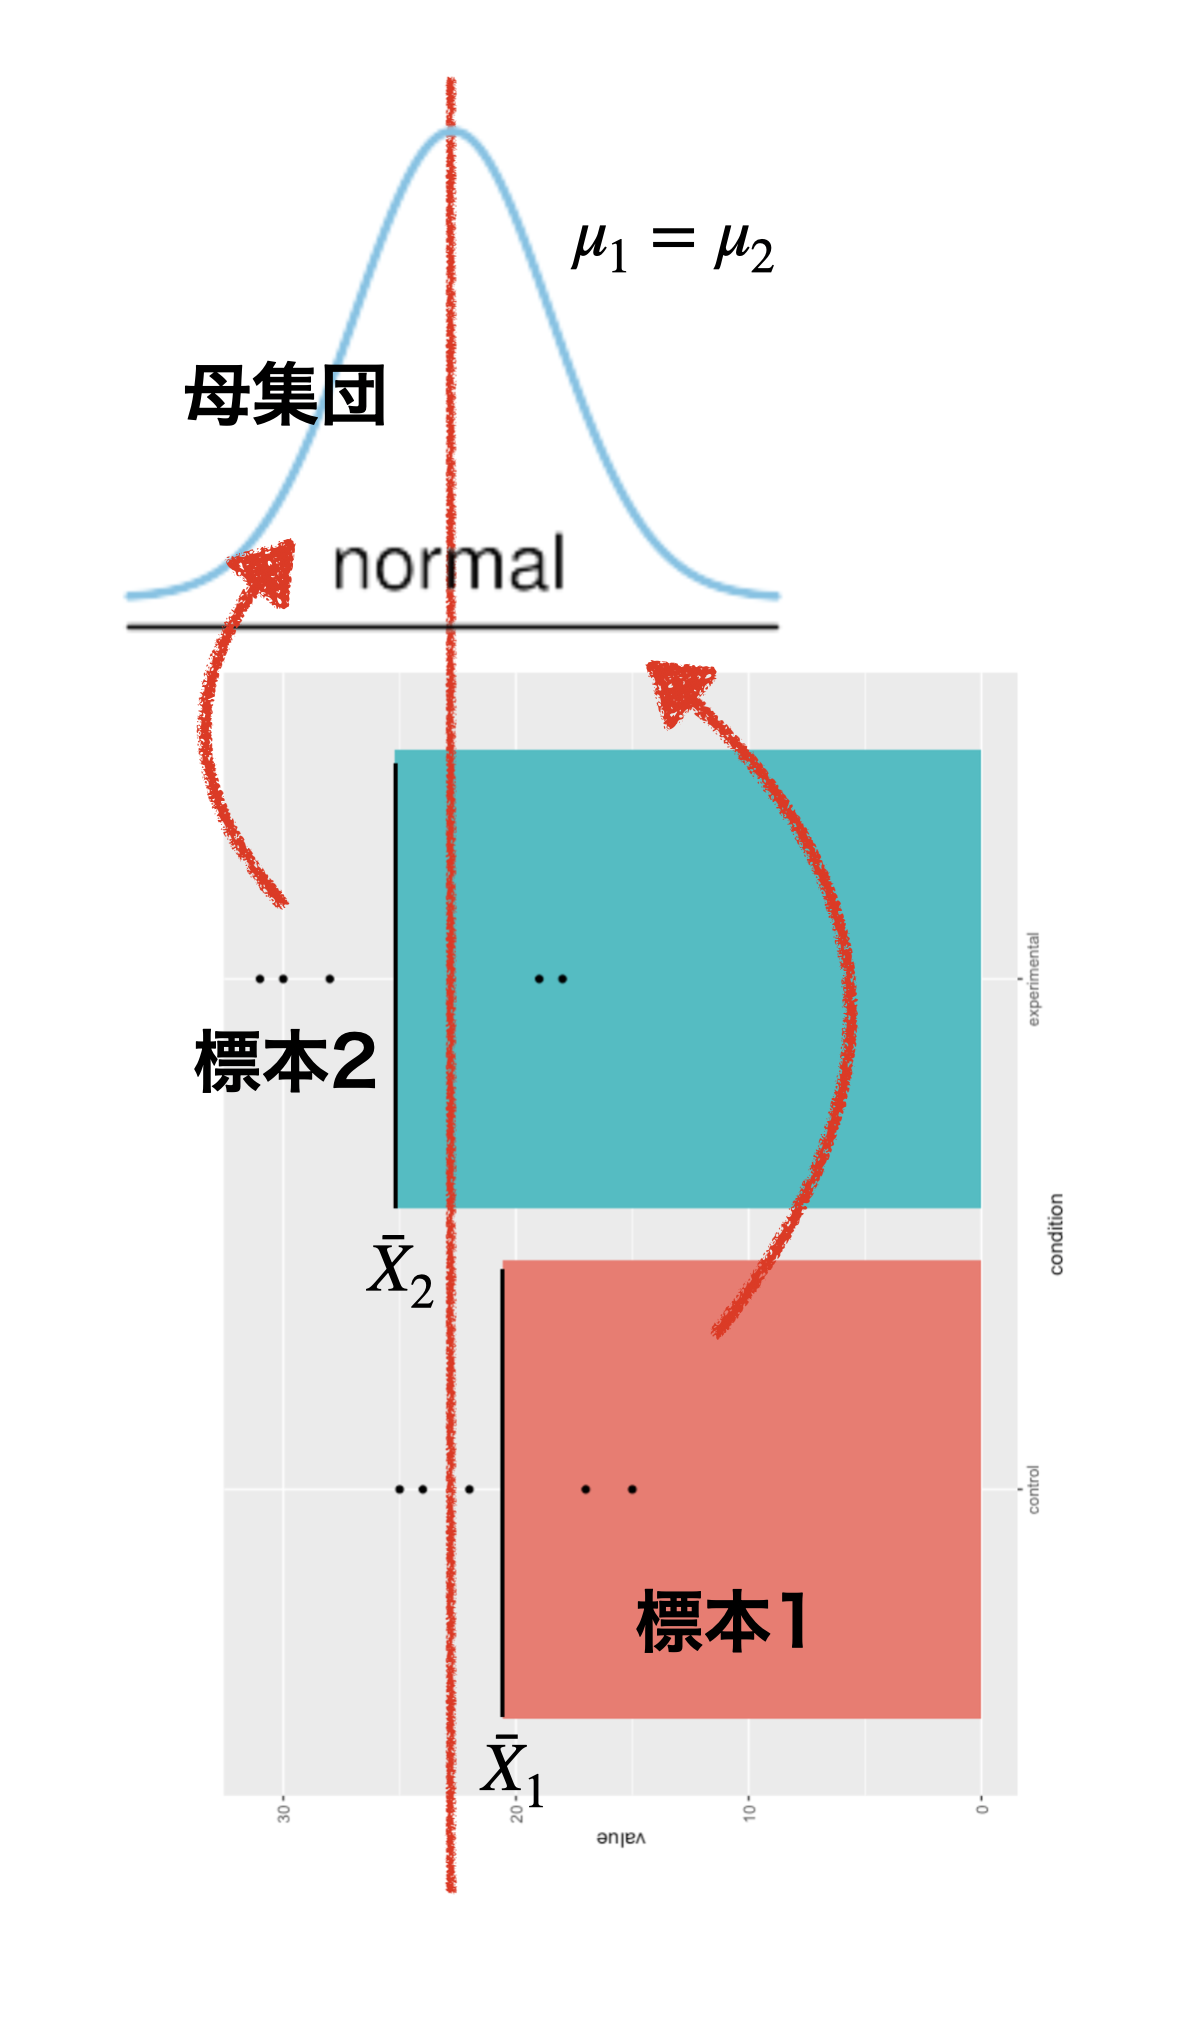
\includegraphics[keepaspectratio,width=8cm]{images/text21/slide21_04.png}
    \caption{母集団が上になるように元の図を回転しています}
    \label{fig::21_04}
\end{figure}

それぞれの標本平均から推定される，母平均の位置は幅を持って推定されますから，その幅がどの程度重複しているのかを考える必要があります。同じだと言えるほど重複しているのか，イエスかノーか，と差し迫った状況では何らかの基準を持って決めないといけませんから，間違って差があると言ってしまう可能性を低く抑えつつ(有意水準$\alpha=0.05$にするのが一般的)，結論を出しましょうというのが帰無仮説検定でしたね。

\subsection{神様の目から見た実験計画}
ここで，同じデータを別の見方で捉えてみましょう。

今回の例において，従属変数である心理変数はどういう特徴なのか，目に見えないものなのでわかりません。でも，心の問題は無数の要因が積み重なった結果であると考えると，正規分布を仮定するのが自然です。つまり，実験群のひとも統制群のひとも，大きな視点から考えれば同じ人間という正規母集団からのサンプルなのです。

さて，実験参加者たちは実験者によって無作為に実験群と統制群に割り当てられました(RCT)。個人差がなければ，各群1名ずつのスコアを比較して考えれば良いのですが，人間を対象にしている以上そうはいきません。個人差がどうしても生じてしまうので，複数人を集めて個人差を相殺することを考えます。各群の平均値の違いを見ることで，操作の効果を見ることにするのです。

もしこの実験に効果がなければ，2群の平均値は同じになるでしょう。この時の平均値は，実験群と統制群に分けた効果がないのですから，両群のスコアを足しあわせた全体平均になるはずです。効果がない=全体平均，なのです。しかし，群ごとに見てみると全体平均から違いが生じています。図\ref{fig::21_03}では，統制群は相対的に低く，実験群は相対的に高い平均値を示しています。この差分こそ(図\ref{fig::21_03}では短い緑の矢印で示しています)，実験の効果なのです。

\begin{figure}[hb]
    \centering
    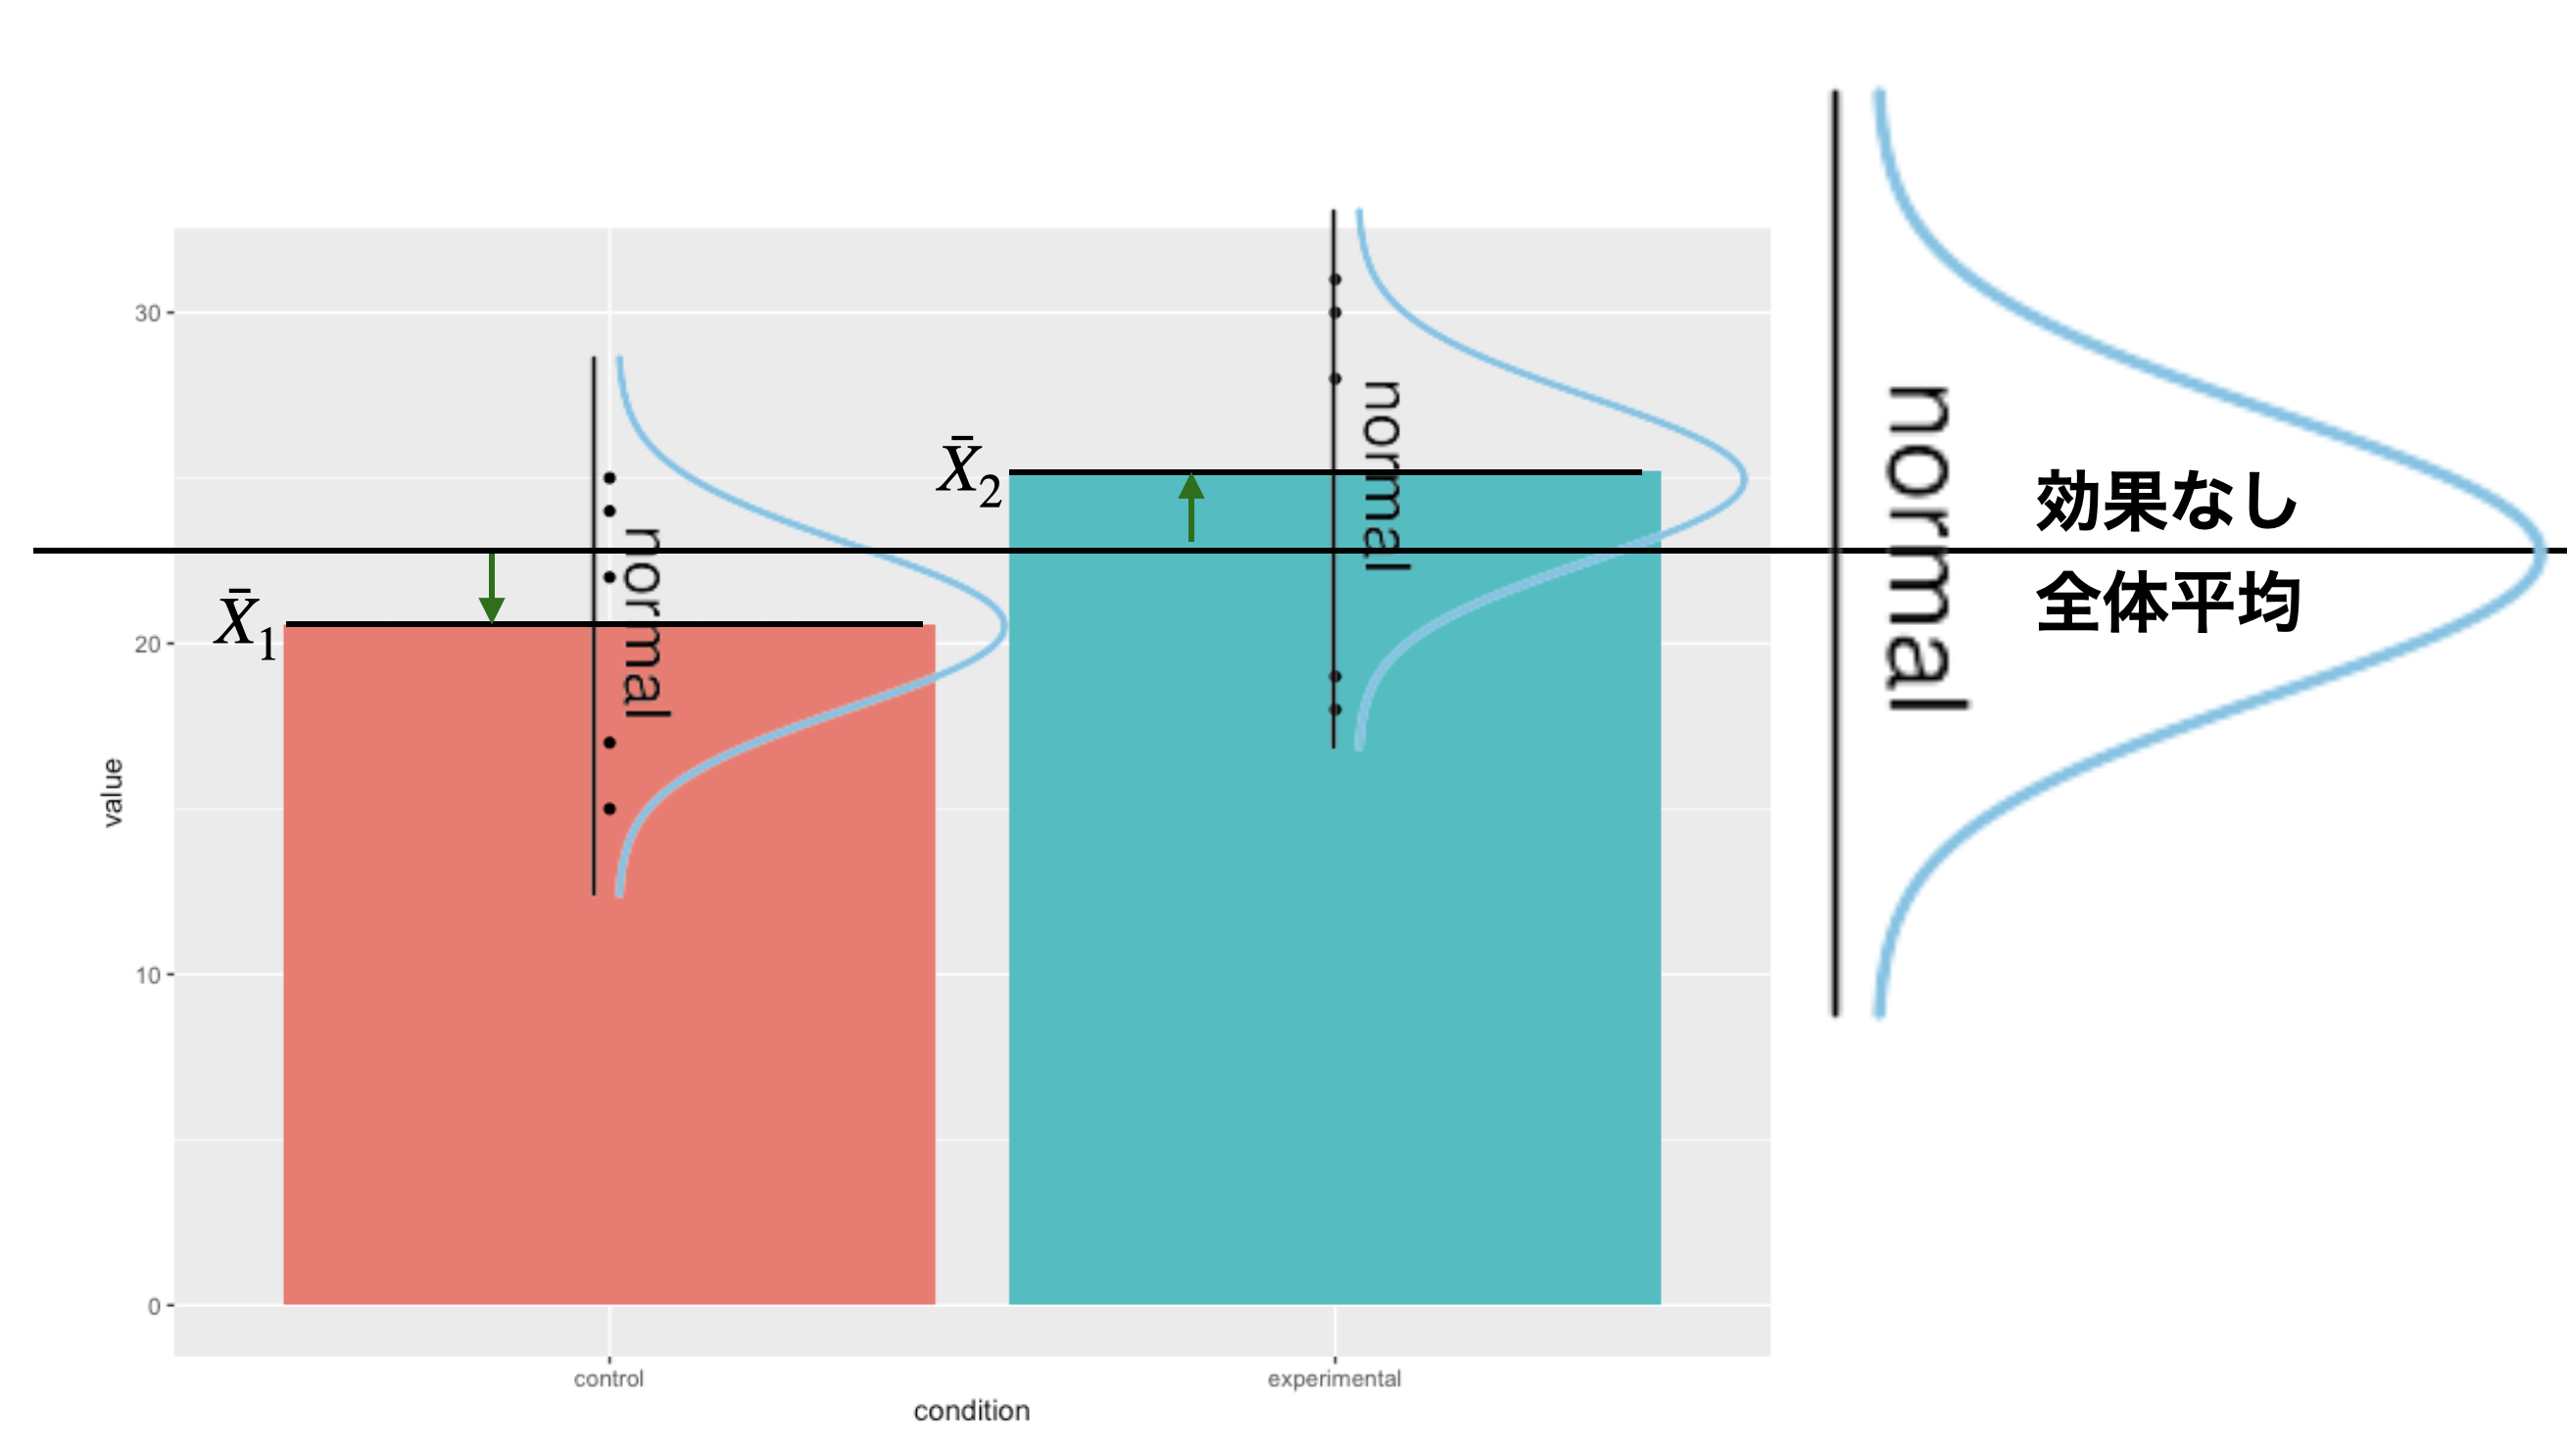
\includegraphics[keepaspectratio,width=12cm]{images/text21/slide21_03.png}
    \caption{効果がなければ全体平均に同じ。群の効果は相対的に平均値をずらす。}
    \label{fig::21_03}
\end{figure}

% このことを，数式的な表現で考えてみたいと思います。
% まず，各群のデータを$X_{ij}$で表します。ここで$i$は実験参加者の番号，$j$は実験群か統制群かを表す記号だと思ってください。仮想データとの対応を表\ref{tbl::21_01}に示しておきます\footnote{ここでのデータは第\ref{chapter19},\ref{chapter20}講の一要因群間2水準の$t$検定データと同じで，表は\ref{tbl::19_02}に少し手を加えたものです。手を加えた部分は，数式表現の列(notation)はもちろんなのですが，IDのところを通し番号から群ごとの番号に変えました。こうすることで，各群$N=5$だな，ということがわかりやすくなったかと思います。}。

% \begin{table}[ht]
%     \centering
%     \caption{仮想データ例と記号の対応} 
%     \begin{tabular}{rlcr}
%       \hline
%     ID & condition & notation & value \\ 
%       \hline
%     1 & control & $X_{11}$ & 25 \\ 
%       2 & control & $X_{21}$& 15 \\ 
%       3 & control & $X_{31}$& 24 \\ 
%       4 & control & $X_{41}$& 17 \\ 
%       5 & control &  $X_{51}$&22 \\ 
%       1 & experimental & $X_{12}$& 31 \\ 
%       2 & experimental & $X_{22}$& 28 \\ 
%       3 & experimental & $X_{32}$& 30 \\ 
%       4 & experimental & $X_{42}$& 19 \\ 
%       5 & experimental & $X_{52}$& 18 \\ 
%        \hline
%     \end{tabular}
%     \label{tbl::21_01}
% \end{table}

% さて，群ごとの平均は次のように書くことができます。
% \[ \bar{X}_1 =\frac{1}{5} \sum_{i=1}^5 X_{i1} \]
% \[ \bar{X}_2 =\frac{1}{5} \sum_{i=1}^5 X_{i2} \]
% また，全体平均次のように書くことができます\footnote{gmはgrand meanの略です。}。
% \[ \bar{X}_{gm} = \frac{1}{10} \sum_{i} \sum_{j} X_{ij} \]
% これは標本を使った平均値ですが，本来は推定したい(群間の差がない)母平均について議論したいところです。$\bar{X}_{gm}$は母平均の推定値として使い道はありますが，理想化・抽象化して語れるのがモデルの良いところですから，ここでは全体平均を未知数を表すギリシア文字$\beta$をつかって$\beta_0$としておきましょう。

% さて次に，群わけの効果を$\beta_1$としましょう。すると各群の平均のモデルは
% \[ \mu_1= \beta_0 + \beta_1 \]
% \[ \mu_2 = \beta_0  -\beta_1 \]
% と表すことができます。左辺も各群の母平均なので，未知数を表すギリシア文字になっています。

% つづいて，ここでの個人差はこの実験で制御できない誤差であり，群平均を中心にどういう向きで出るかわからないものですから，このことを表現するなら，
% \[ X_{ij} = \mu_j + \epsilon_{ij} \]
% ということになります。これらを組み合わせると，
% \[ X_{i1} = \beta_0 + \beta_1 + \epsilon_{i1} \]
% \[ X_{i2} = \beta_0 - \beta_1 + \epsilon_{i2} \]
% と書くことができます。ここで一工夫。$\beta_1$にプラス，マイナスの符号がついているのは，$+1,-1$を掛け算していると考えてみましょう。この符号を決めているものを$X_{1}=+1,X_{2}=-1$と表したとすると，まとめて次のように書くことができます。
% \begin{equation}
%     \label{eq::21_1}
%      X_{ij} = \beta_0 +  \beta_1 X_{j} + \epsilon_{ij} 
% \end{equation}
% これ，どこかで見覚えありませんか。そうです，前期の間にやった回帰分析と同じ形をしているのです($\to$第\ref{chapter8}講参照)。

% 回帰分析を今ここで大雑把に復習しておきますと，2つの変数$x_i,y_i$があったときに，両者の間に何らかの関数関係がある，と考えましょうという話でした。関数関係とは，一方を定めれば他方も定まるという関係ですから，この関係を数式で表現してやれば予測もできるぞ，嬉しいぞ。ということで，最も簡単な関数関係って何だ？そう，中学校の時にやった一次関数$y=ax+b$だよね，ということでした。ただ中学校の時の話とは違って，データがたくさんあり，かつ，全部にぴったり当てはまる線は引けない。なので，ちょっと誤差はあるけどだいたいあってる線を引こうね，ということを考えたのでした。この関数(一次関数，線形関数，線形モデル)で予測される値を$\hat{y}_i$と表したとすると,

% \[ \hat{y}_i = b_0 + b_1x_i \]
% データ$y_i$は予測値$\hat{y}_i$に誤差$e_i$がついて現れるから，
% \[ y_i = \hat{y}_i + e_i  \]
% なので，これを統合して
% \[ y_i = b_0 + b_1 x_i + e_i \]
% としたのでした。

% さてさて。記号で$y_i,x_i$とか$b_0,b_1$だったのが$\beta_0$とか$\beta_1$などと変わってはいますが，基本的には$y=ax+b$の一次線形関数の形です(図\ref{fig::21_05})。
% \begin{figure}[ht]
%     \centering
%     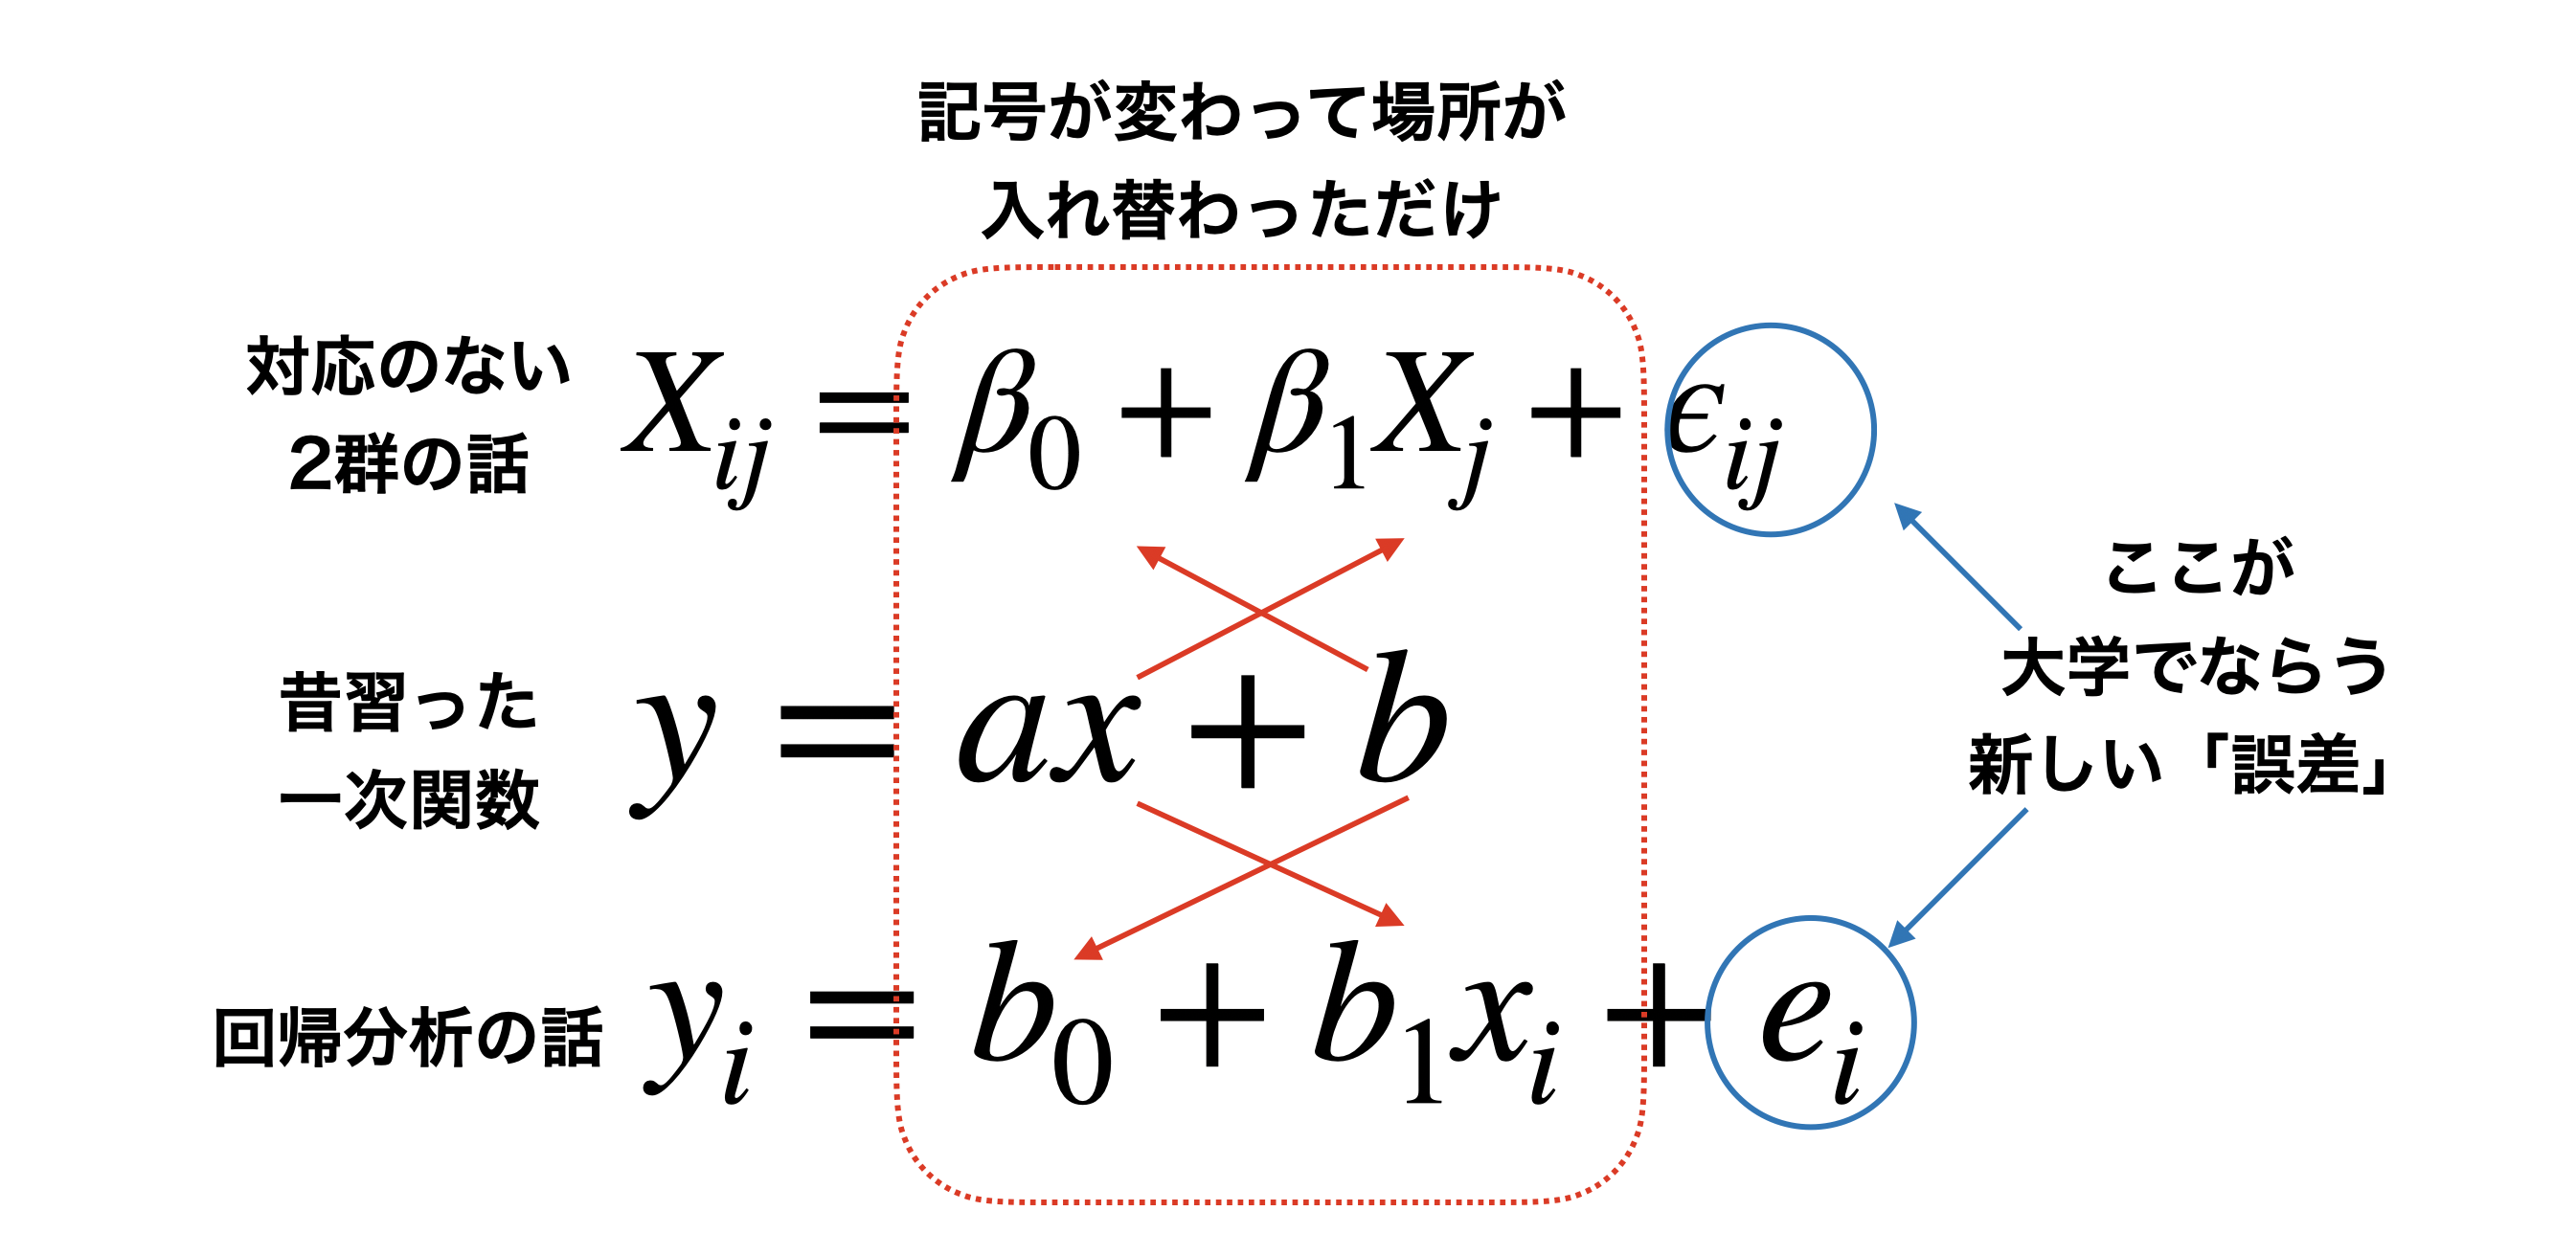
\includegraphics[keepaspectratio,width=12cm]{images/text21/slide21_05.png}
%     \caption{数学的には記号が変わっても使われ方が同じであれば同型と考えます}
%     \label{fig::21_05}
% \end{figure}


% 先ほど，効果がない＝全体平均，という言い方をしました。効果のことを，記号$\beta_1$で表しているのですから，効果がないというのは$\beta_1=0$ということです。そうすると$\beta_1X_j$ の項が消えてしまいます。つまり，全体平均$\beta_0$に誤差$\epsilon_{ij}$がついただけで，データは1つの正規分布から出てきたまま，ということになります。

1つの共通の正規分布。2つの群に分かれない，同じ正規分布。そろそろ帰無仮説検定と繋がってきたのではないでしょうか。効果がない，というのはまさに，帰無仮説のことですよね。つまり帰無仮説は，$\beta_1=0$という傾きゼロの直線，図\ref{fig::21_03}では群平均を横切っている，横一線の線形モデルだったのです。平均値の差の検定というのは，群平均が横一直線＝傾きゼロではないよ，という結論を出すためのロジックであり，比較される対立仮説は「傾きゼロでない何か」というモデルです。繰り返しになりますが，帰無仮説が傾きゼロという一点ばりに対し，対立仮説はゼロ以外であれば何でも良いという非常に非対称な戦いであり，結論が出たからと言って「じゃあゼロでない，何なのか」ということまでは強く主張できません。帰無仮説検定は補助的に使いつつ，実質はどのように傾いているのか，差の信頼区間はどの程度あるのか，効果量(標準化された平均値の差)は大きいのかといった，実質的な大きさを考えることが重要です。

また，前期の回帰分析の時は最小二乗法を使って回帰係数を求めたのでした。ただ，その時は推測統計学的な発想を導入していませんでした。データに最もうまく適合するために計算すると，とにかく求められるよ，という説明の仕方だったかと思います。手元のデータの話，つまり標本の話しかしていませんでしたので，係数として$b_0,b_1$と書いていたのですが，推測統計学の枠組みでこれを考えると，我々が知りたいのは母集団における傾き，母数だということになりますので，今回ギリシア文字$\beta_1$とか$\epsilon_{ij}$とします。

平均値差の検定と回帰分析は同じものなのだ，という話をしてきました。いずれも正規分布を仮定しており，その意味が「心理現象に仮定される全体傾向をあらわす分布」なのか「誤差の分布」なのか，という微妙な出自の違いを持っていると言えるかもしれません。しかし数学的には同じことなので，どちらの筋道からでも考えて，同じように利用できます。

また，回帰分析の係数を最小二乗法で求めたように，推測統計の枠組みで平均値を推定するのに最小二乗法を使うのだろうか，と考えている人もいるかもしれません。実はこれが大変興味深いところなのですが，推測統計の枠組みでは正規分布という確率分布を利用しますから，誤差を最小にしようという解析的な(確率的でない，という意味でつかています)方法とは異なる考え方を使う必要があります。確率分布を使った母数の推定方法として，\keyterm{最尤法}{さいゆうほう}{Maximum Likelihood metod}と\keyterm{ベイズ法}{べいずほう}{Bayesian metod}という二種類の方法を今後説明していきますが，結論だけ先にいっておくと，幸いにして最小二乗法による答えと最尤法による答えは\textbf{ぴったり一致します}。

ちなみにこれまでやってきた，標本平均や標本分散から母数を推定する方法は，「モーメント法」というやり方に分類されます。何であれ，同じデータであれば推定値はだいたい同じになります。同じものを推定しようとしてるのですから，違ってきたらむしろ困りますわね。

\section{一要因Betweenデザイン，多水準の場合}
これまでは2水準の平均値の比較について話をしてきましたが，3水準以上になるとどうなるのでしょうか？
これも，基本的には線形モデルの延長で考えることができます。例えば表\ref{table::21_02}のようなデータがあったとしましょう。要因は1つですが水準は3つで，群間デザインの例です。
\begin{table}[ht]
    \centering
    \caption{一要因3水準Between計画のデータ}
    \begin{tabular}{rccr}
      \hline
    id & condition & notation & value \\ 
      \hline
      1 & 1 & $X_{11}$ & 6 \\ 
      2 & 1 & $X_{21}$ & 6 \\ 
      3 & 1 & $X_{31}$ & 5 \\ 
      4 & 1 & $X_{41}$ & 5 \\ 
      1 & 2 & $X_{12}$ & 7 \\ 
      2 & 2 & $X_{22}$ & 4 \\ 
      3 & 2 & $X_{32}$ & 7 \\ 
      4 & 2 & $X_{42}$ & 6 \\ 
      1 & 3 & $X_{13}$ & 4 \\ 
      2 & 3 & $X_{23}$ & 3 \\ 
      3 & 3 & $X_{33}$ & 4 \\ 
      4 & 3 & $X_{43}$ & 6 \\ 
       \hline
    \end{tabular}
    \label{table::21_02}
    \end{table}
それぞれの群平均は，$\bar{X}_1 = 5.5,\bar{X}_2 = 6.0,\bar{X}_3 = 4.25$であり，全体平均は$\bar{X}_{gm}= 5.25$になります。
帰無仮説検定の文脈で考えれば，帰無仮説は「母平均に差がない」という仮説になりますから，記号で言えば$\mu_1 = \mu_2 = \mu_3$になります。
線形モデルで考えれば，図\ref{fig::21_06}にあるように，傾きのない線形モデル，つまり$X_{ij} = \bar{X}_{gm} + \epsilon_{ij}$の横一線ということになります。

\begin{figure}[ht]
    \centering
    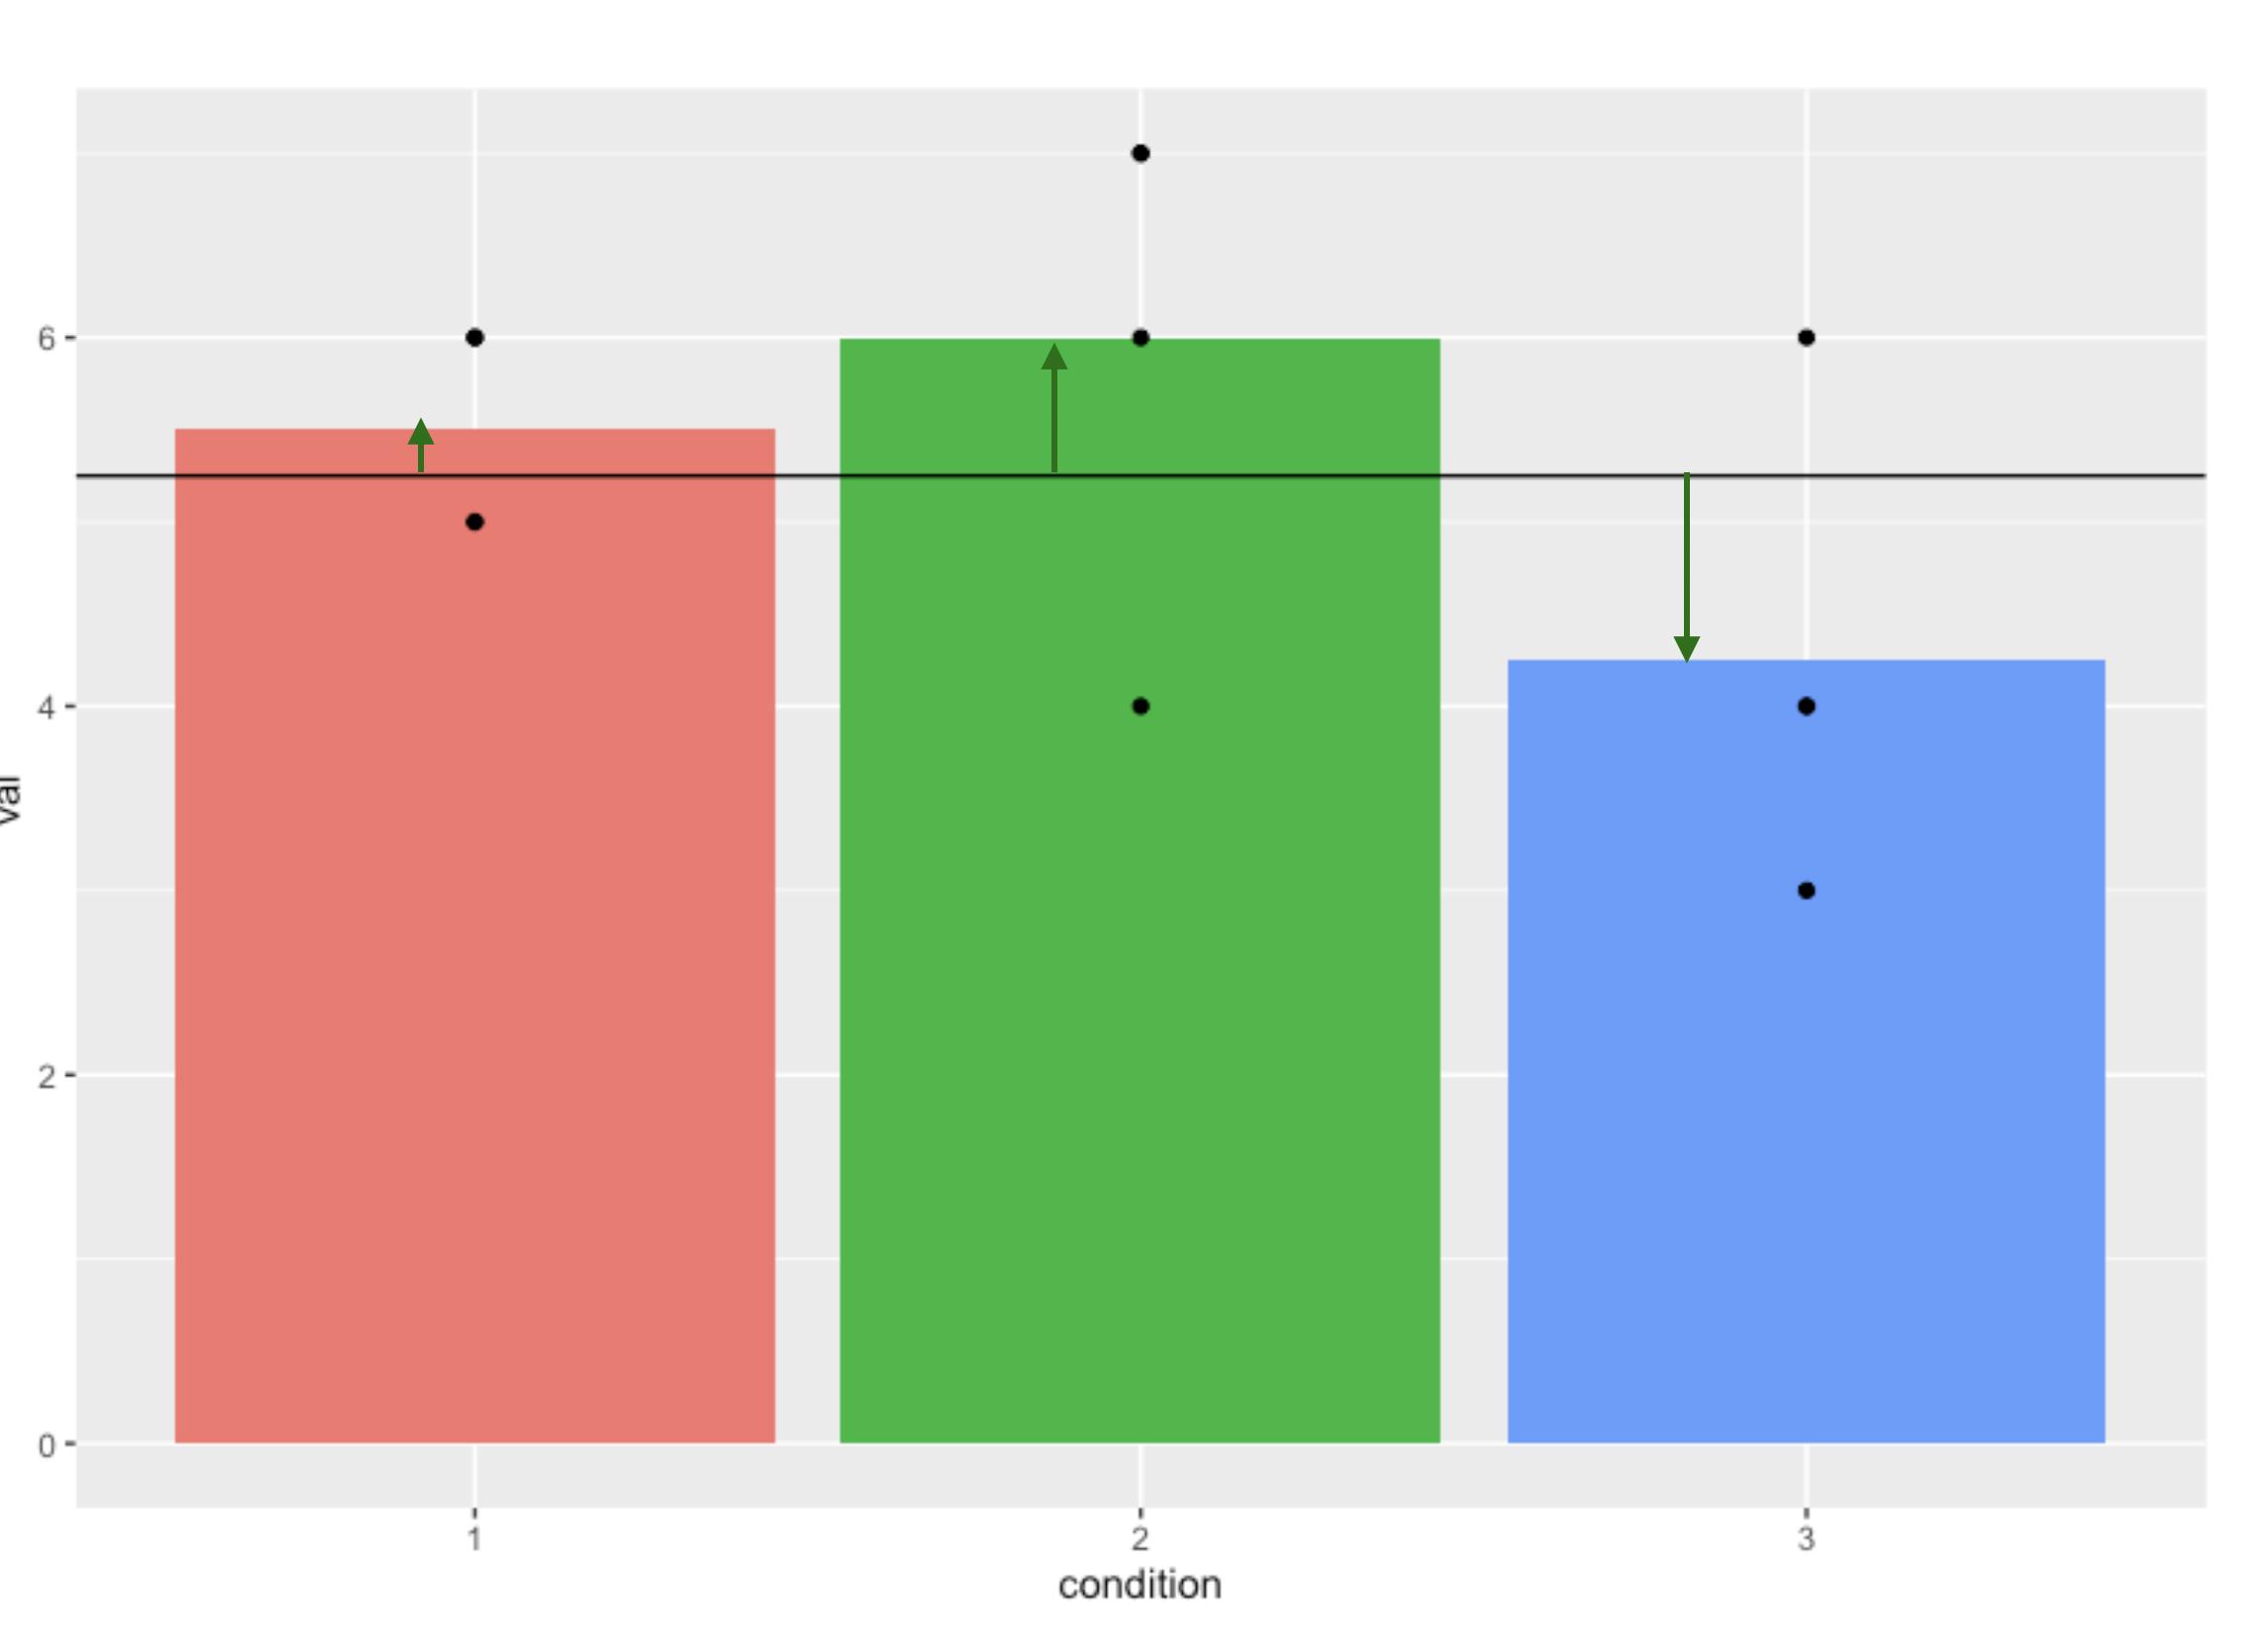
\includegraphics[keepaspectratio,width=12cm]{images/text21/slide21_06.png}
    \caption{表\ref{table::21_02}を可視化したもの。全体平均からの矢印は群効果の大きさ}
    \label{fig::21_06}
\end{figure}

対立仮説は帰無仮説の否定ですから，横一線の直線ではない(傾きがある)，あるいは母平均のどこかに差がある，というものになります。横一線ではない，という話ではありますが，右上がりの直線なのか，左下りの直線なのか，という話は一概にできないことに注意してください。というのも，横軸の水準1/2/3は名義尺度水準に過ぎないからです。水準1/2/3が「統制群」「操作Aをした群」「操作Bをした群」であったとして，統制群が1である理由は特になく，2でも3でも構いません。\underline{名義尺度水準は，対象と数字が一対一対応している}ことがその要件であって，数字の並びに意味がないからです。図\ref{fig::21_06}を見ると，水準1から2に向けては右上がり，水準2から3に向けては右下がりになって，一本の直線では表現できないですね。ただこれの並びを変えて，水準3/1/2の順番にすると右上がりの直線をあてがうことが可能です(図\ref{fig::21_07})。もちろん水準2/1/3の順にして右下がりの直線を当て嵌めても構いません。いずれもデータの持つ情報は同じです。ですから，対立仮説としては「横一線ではない」「母平均が同じではない」とするに留めましょう。

要因計画に帰無仮説検定の要素を加えた分析方法を特に，\keyterm{分散分析}{ぶんさんぶんせき}{Analysis of Variance}と呼びます。\textbf{ANOVA}(アノーバ)と略して言われることもあります。「分散」分析といっていますが，やっていることは「平均値差の検定」です。どうして分散と呼んでいるのかは，直線が右上がりなのか，右下がりなのか一概に決められないことと関係があります。プラスにもマイナスにも変動するので，符号の効果をなくすべく二乗することで計算を進めるからです。

\begin{figure}[ht]
    \centering
    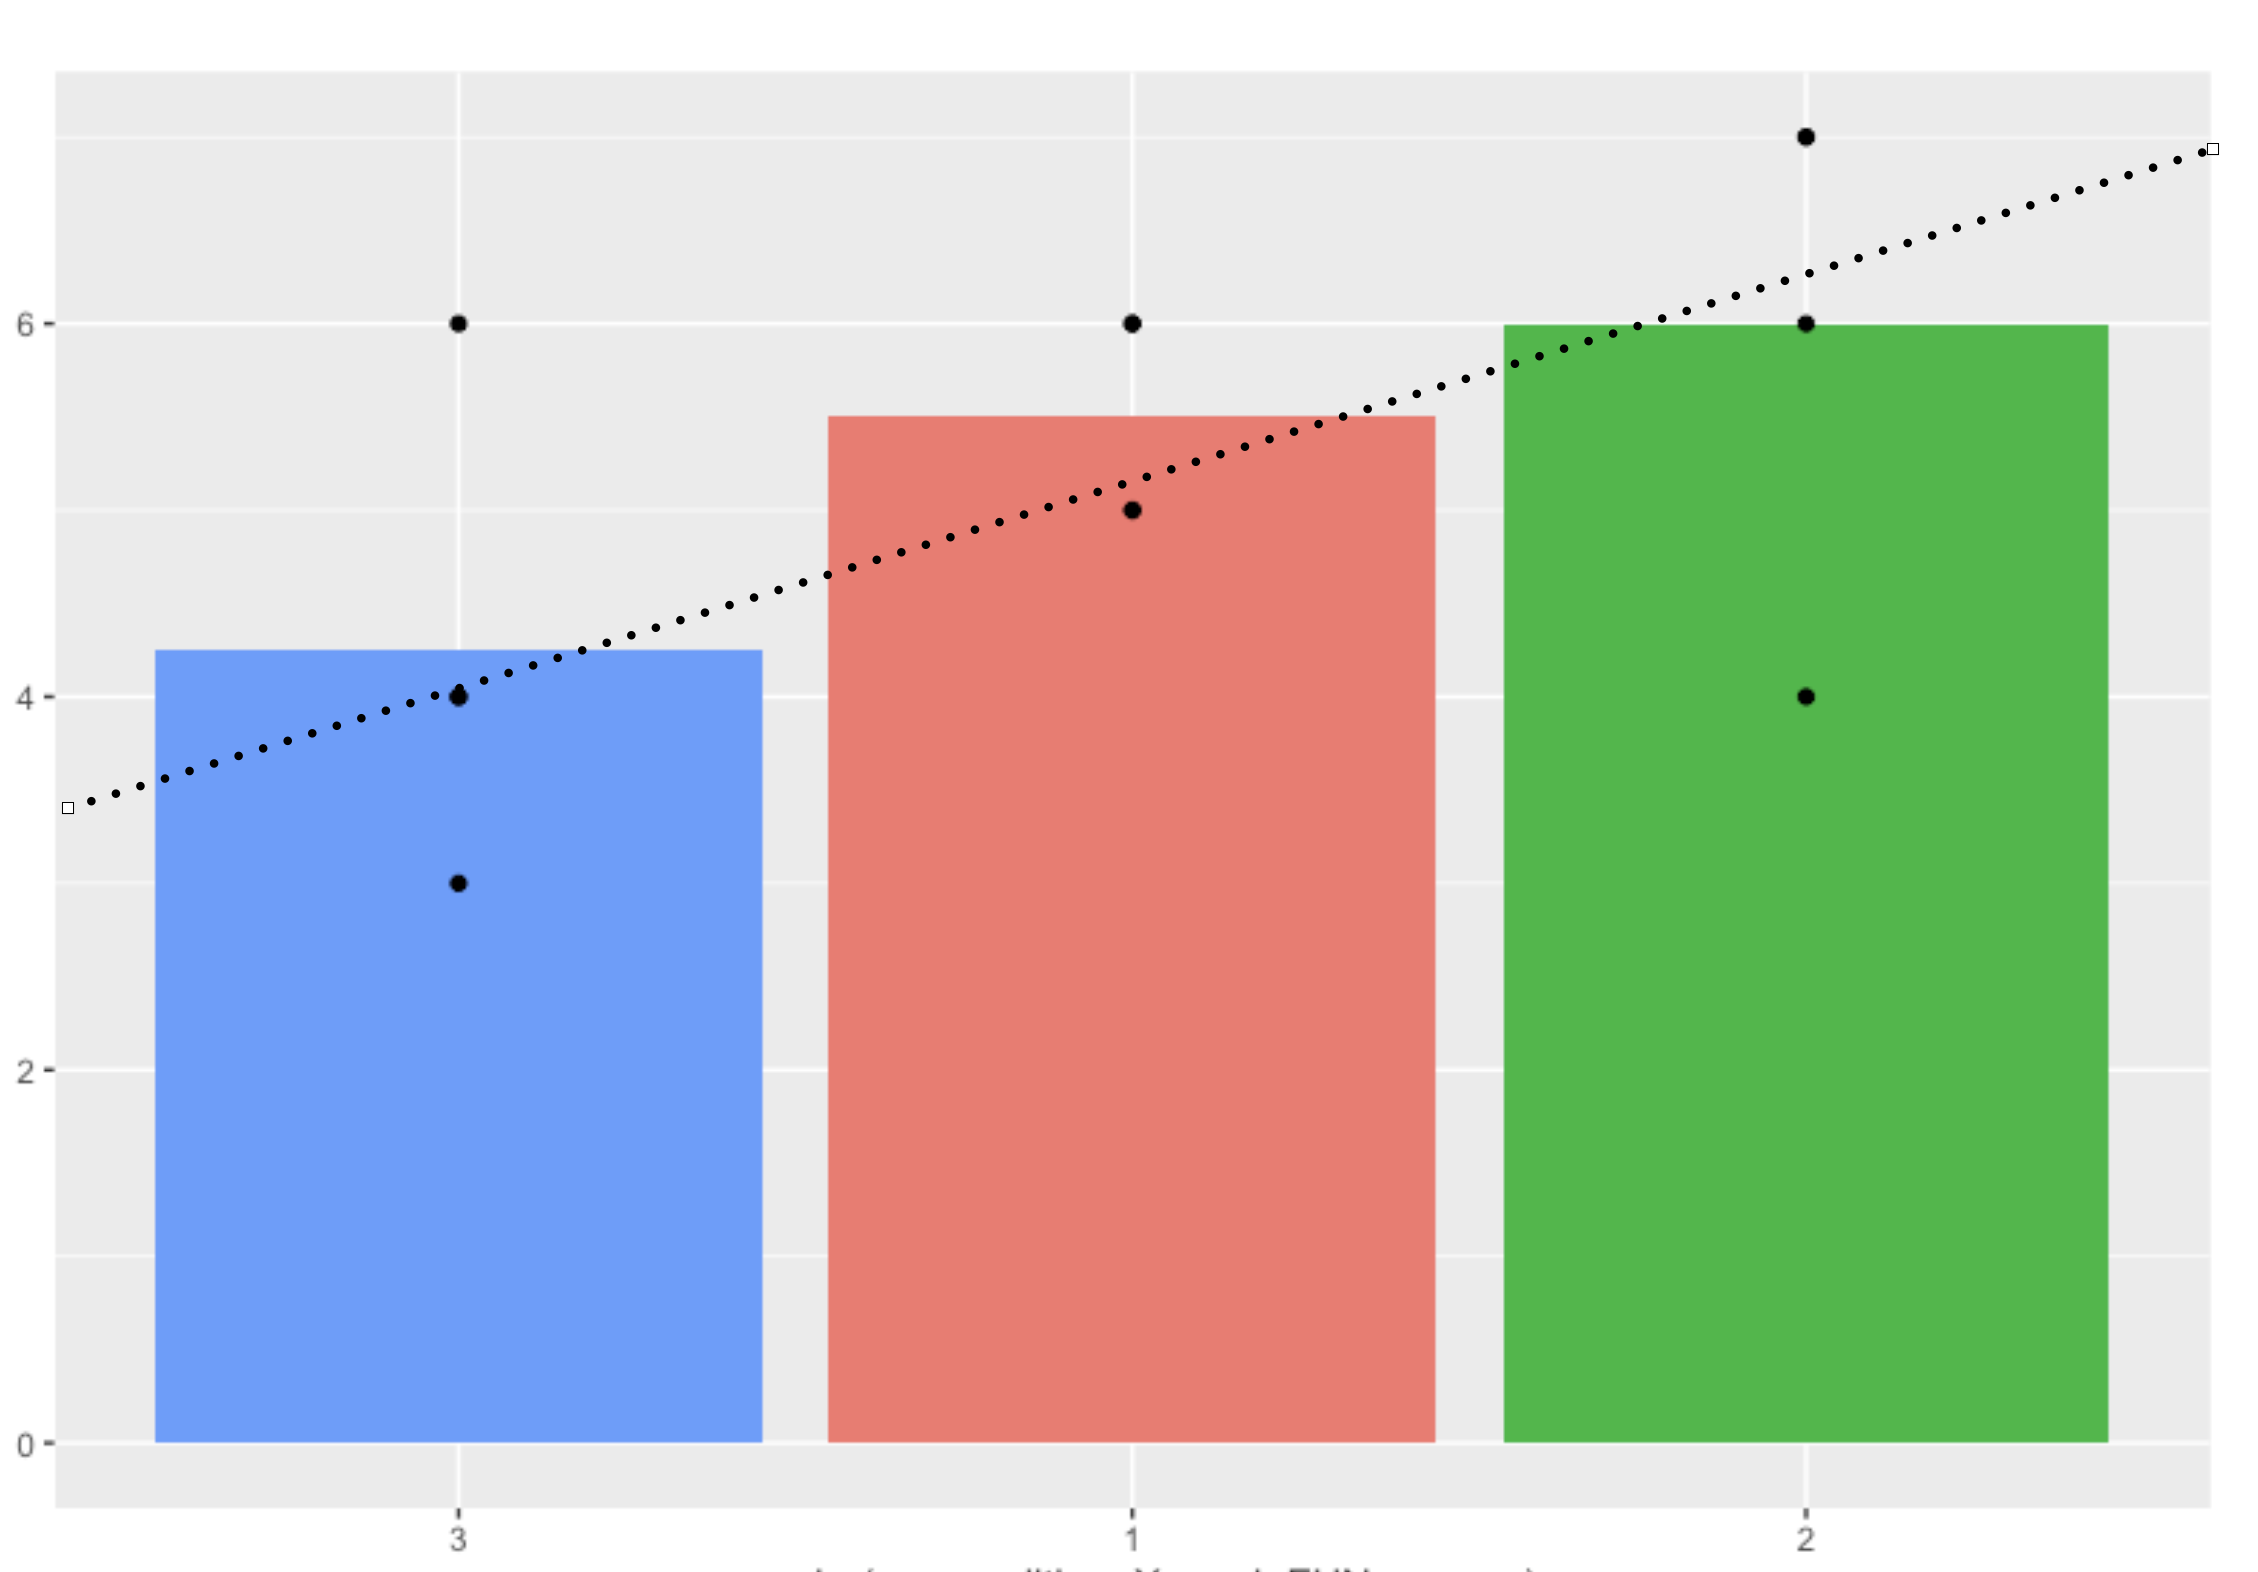
\includegraphics[keepaspectratio,width=12cm]{images/text21/slide21_07.png}
    \caption{横軸は並べ替えても構わない}
    \label{fig::21_07}
\end{figure}

さて，前期の間は二乗して効果の大きさを算出するところまではやったのですが，効果と誤差をどうやって比較するか，ということについては伏せたままでした。
というのも，推測統計学的な枠組みがなければ比較方法に言及できず，また帰無仮説検定の枠組みがなければ判断基準に言及できなかったからです。今ではこれらを使って説明できます。すなわち平方和がどのような分布に従うのかを考え，理論分布から統計量を計算すれば良いわけです。その方法についてみていくことにしましょう。
%%%%%%%%%%%%%%%%%%%%%%%%%%%%%%%%%% →Dkiso1_12.texにもらっていきます(2021.05.14)
% \section{線形モデルとしてみた一要因多水準計画}
% まずは線形モデルとして，一要因多水準の要因計画を見るとどう解釈できるかを説明します。ポイントは\underline{平方和の分解}と\underline{分散の比による比較}です。

% \subsection{平方和の分解}
% 群わけされてないデータ全体を考えてみてください(表\ref{tbl::21_01}のvalue列がそうです)。全体平均は5.25，全体の不偏分散は 1.659です。この全体平均は，帰無仮説的な状態，つまり群わけの効果がなく全部が1つの平均値になるならば，というラインです。言い換えると効果とか個性(誤差)がなければ，全ての数字が5.25だったはずなのです。ですが，実際の数字は6($=X_{11}$ほか)とか3($=X_{32}$)といった数字です。この違いを生んでいるのが何なのか，を考えるヒントが分散の中に埋め込まれているはずなのです\footnote{言い方を変えると，分散がゼロであれば何の情報も得られないのでした。テストが全員同じ点だったら，何が原因で成績が上がるのかがわかりません。同じスコアにしかならないんだから。これだとやる気が生じないでしょう?}。なので分散分析では，この分散を分解することを考えます。

% ところで，分散は「平均からの差(平均偏差)」の「二乗」を「平均する(総和して足した数で割る)」という3ステップで計算します。分散分析では最後の「足した数で割る」の箇所を取り除き，平均偏差の二乗和(Sum of Squares, SS)で考えます。実質的に分散と同じ情報を持っている数字です。この「平均からの差」こそ，今探している情報そのものです。これがゼロなら全体平均に一致しますし，分散もゼロになるからです。

% 具体的な数字で考えてみましょう。3つの群それぞれの平均を考えてみます。
% 実験者によって群に分けるという介入がなければ，全員のスコアは5.25だったはずなのでした。しかし，第1水準の平均は5.5になっています。つまり，ここの群に入ると平均で$5.5-5.25=0.25$のプラスの効果が出てくるということです。逆に第3水準の平均は4.25ですから，ここの軍に振り分けられると平均で$4.25-5.25=-1.0$のマイナスの効果が出てくるということになります。このように，全体平均と群平均の差が「群わけの効果」であると言えるわけです。

% さらに細かくみてみましょう。$X_{11}$は，第1水準の群に入れられた人ですから，+0.25の効果が出ているはず。全体平均が5.25でプラス0.25の効果なので，5.5であるべき人なのですが，実際の観測値は6です。この$6-5.5=0.5$の差，これは実験の群わけによる効果ではないので個人差だ，ということになります。ここでは実験外の要因ですから個人差＝誤差と言って良いでしょう。

% これを少し数式で表現しておきます。データは$X_{ij}$で，第$j$群の第$i$番目の人を表すのでした。このデータは，全体平均$\beta_0$と，群の効果(これを$\beta_j$と表しましょう)と個人差に分解できるということで，式で表すと次のようになります。
% \[ X_{ij} = \beta_0 + \beta_j + \epsilon_{ij} \]
% ここで全体平均$\beta_0$の推定値をデータから$\bar{X}_{gm}$とすると，効果$\beta_j$の推定値は
% \[ \beta_j  = \bar{X}_j - \bar{X}_{gm}\]
% で計算できます\footnote{話を単純化するために，効果の項は一つの記号$\beta_j$で代表させていますが，本当はこれにも符号を表現する係数$X_j$をつけて$X_{ij}=\beta_0 + \beta_{1j} X_j + \epsilon_{ij}$とすることで話の一貫性を持たせることができます。ただ，今回は水準が3つあるので$\beta_{11}+\beta_{12}+\beta_{13}=0$という「効果の平均は$0$，相対的に考える」という条件と合わせて考えると，$X_j$をうまく一文字で表すのに困るのです。これは行列表現を使うことで解決できる(し，もっと利点がある)のですが，それは2年次のデータ解析応用の授業で扱う予定です。}。

% 記号だと分かりにくいかもしれませんが，データで考えると表\ref{table::21_03}のようになります。
% \begin{table}[ht]
%     \centering
%     \caption{一要因3水準Between計画のデータを分解する}
%     \begin{tabular}{rccrrrr}
%       \hline
%     id & condition & notation & value($X_{ij}$) & 全体平均($\bar{X}_{gm}$) & 群の効果($\beta_j$) & 誤差($\epsilon_{ij}$)\\ 
%       \hline
%       1 & 1 & $X_{11}$ & 6 & 5.25 & $+0.25$ & $+0.50$\\ 
%       2 & 1 & $X_{12}$ & 6 & 5.25 & $+0.25$ & $+0.50$\\ 
%       3 & 1 & $X_{13}$ & 5 & 5.25 & $+0.25$ & $-0.50$\\ 
%       4 & 1 & $X_{14}$ & 5 & 5.25 & $+0.25$ & $-0.50$\\ 
%       1 & 2 & $X_{21}$ & 7 & 5.25 & $+0.75$ & $+1.00$\\ 
%       2 & 2 & $X_{22}$ & 4 & 5.25 & $+0.75$ & $-2.00$ \\ 
%       3 & 2 & $X_{23}$ & 7 & 5.25 & $+0.75$ & $+1.00$\\ 
%       4 & 2 & $X_{24}$ & 6 & 5.25 & $+0.75$ & $+0.00$\\ 
%       1 & 3 & $X_{31}$ & 4 & 5.25 & $-1.00$ & $-0.25$\\ 
%       2 & 3 & $X_{32}$ & 3 & 5.25 & $-1.00$ & $-1.25$\\ 
%       3 & 3 & $X_{33}$ & 4 & 5.25 & $-1.00$ & $-0.25$\\ 
%       4 & 3 & $X_{34}$ & 6 & 5.25 & $-1.00$ & $+1.75$\\ 
%        \hline\hline
%        合計 &&&&& 0.00 & 0.00\\\hline
%     \end{tabular}
%     \label{table::21_03}
%     \end{table}
% この表\ref{table::21_03}，「全体の平均」の列は全部同じです。群わけがなければ，全員5.25だったはずだ，と言うわけです。次に「群の効果」列を見てもらいたいのですが，これは3つの群(condition列に対応)ごとに同じです。また，これは相対的な大きさなので，全部足し合わせるとゼロになります。最後に誤差の列。これの計算は$\epsilon_{ij} = X_{ij} - \bar{X}_{gm}-\beta_j$でできます。

% このように，平均からの差を考えると，効果あるいは誤差が計算できることになります。ただし，効果や誤差はプラスであったりマイナスであったりしますから，影響力の大きさとして比較できません。最後の合計欄にあるように，全部足し合わせるとゼロになってしまうのです。そこで，これを二乗して(平均偏差の平方和にして)，比較することを考えます。

% 分散分析の最初のポイント，平方和の分解とは，全体の平方和を「効果」と「誤差」に分解することである，というのがご理解いただけましたでしょうか。
% \subsection{分散の比による比較}
% 次はこれの比較です。以前，「差があるとはどう言うことか」で説明したように($\to$セクション\ref{fig::ch11D_133})，群に分けたことによって生まれた違いは，個人差の違いと比較して初めてその効果を明確にできます(図\ref{fig::21_08}に再掲)。この考え方は，効果量の話とも一貫するものです。

% \begin{figure}[ht]
%     \centering
%     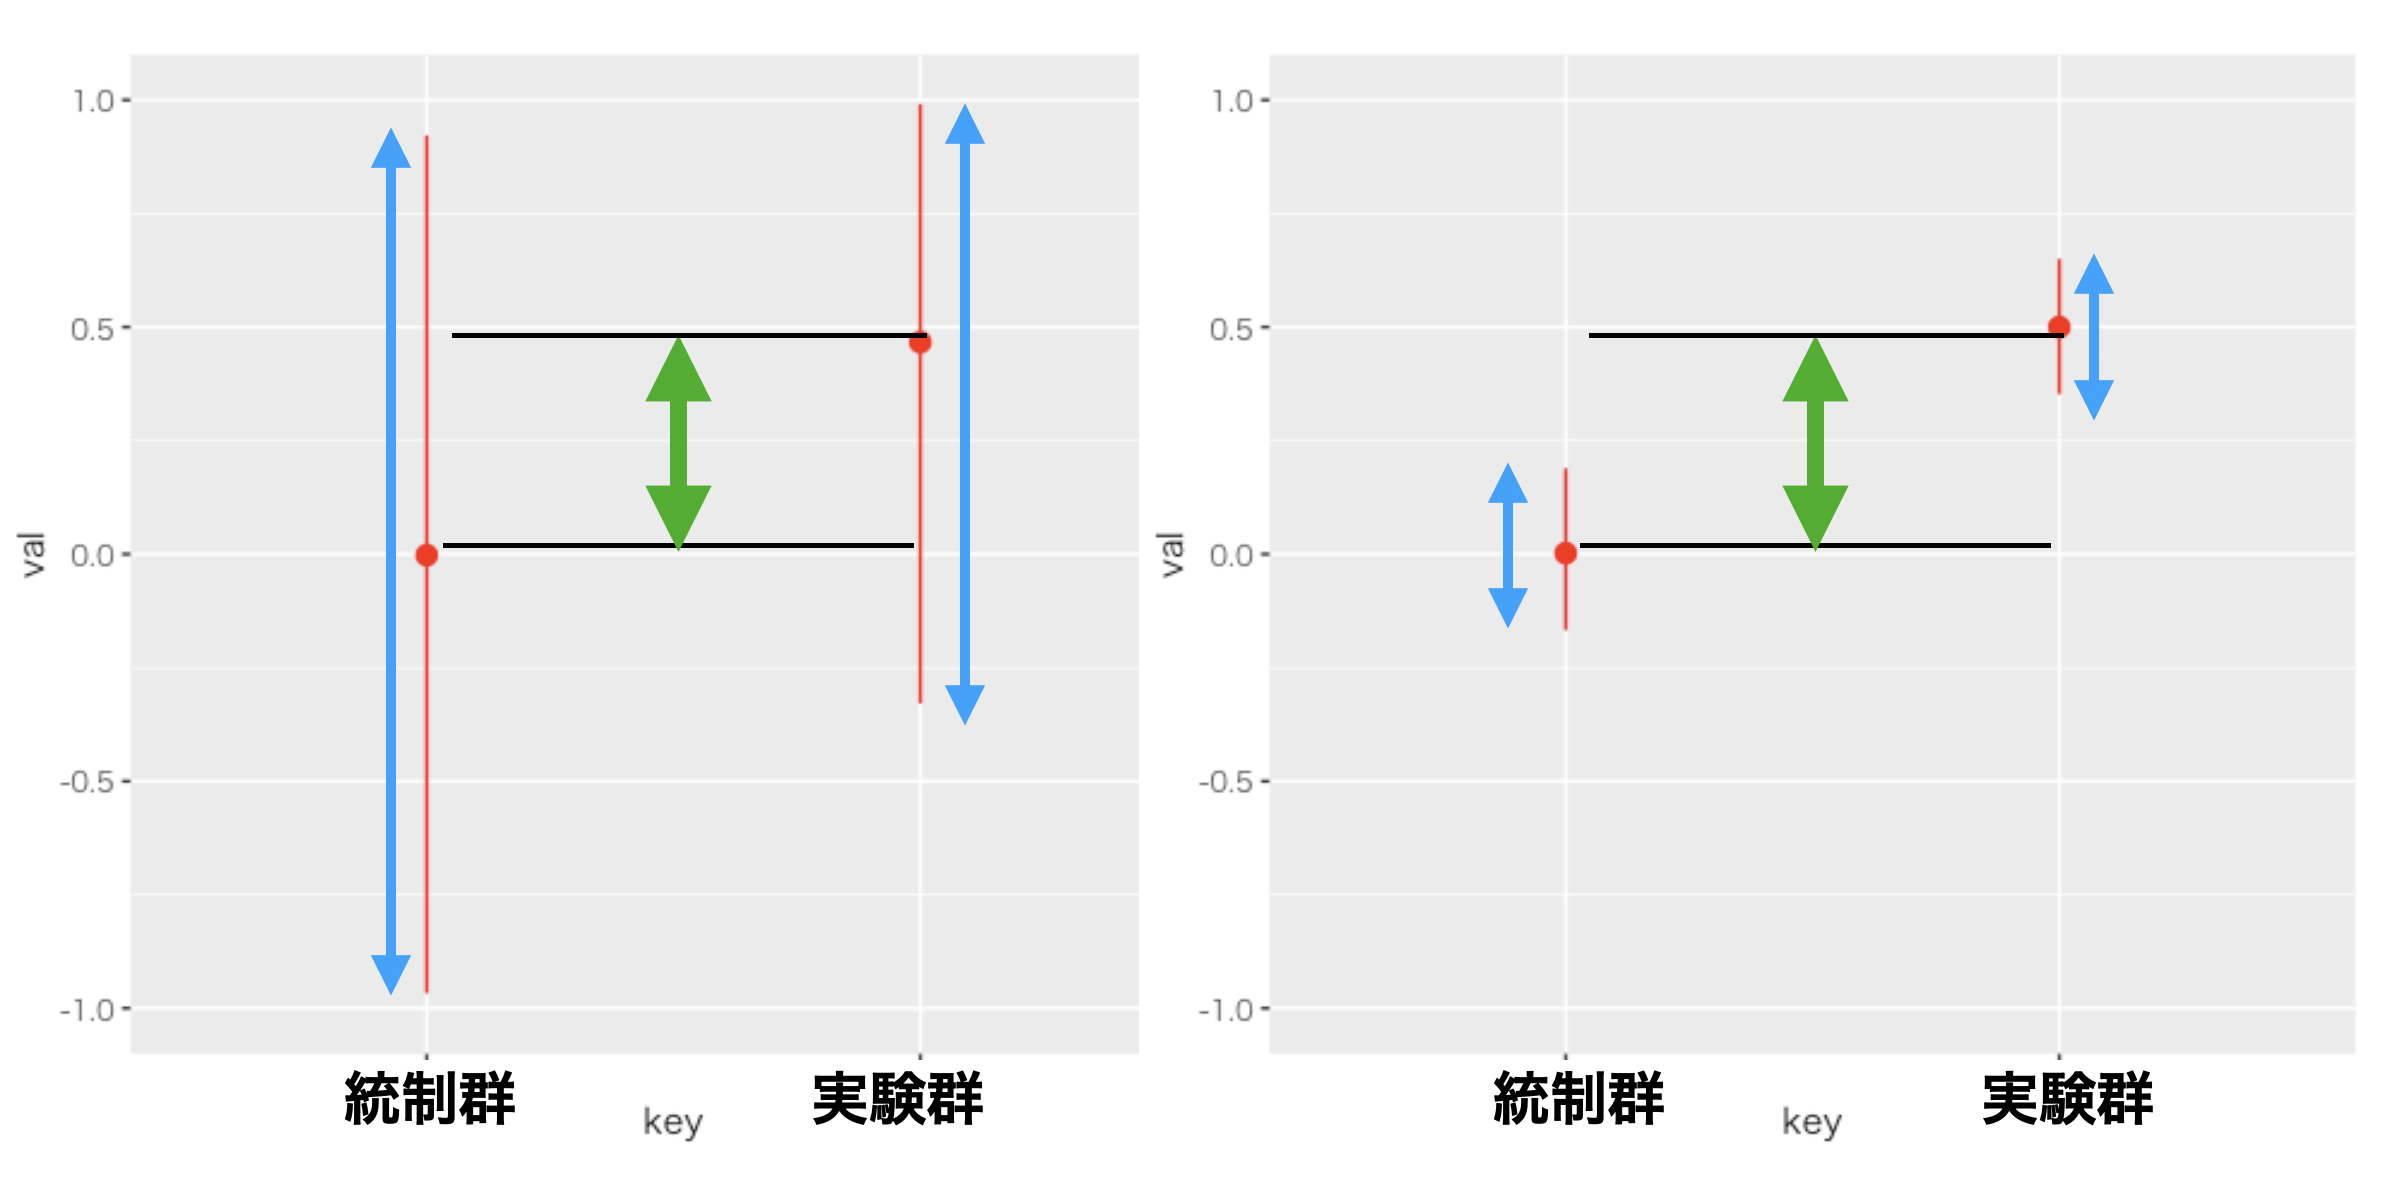
\includegraphics[keepaspectratio,width=12cm]{images/text21/slide21_08.png}
%     \caption{平均値の差(群の効果)が同じ二つの実験の例。左側は群間の分散(緑の矢印)に比べて群内の分散(青の矢印)が大きいため，効果があるとは言いにくい。右側の例では，統制群の最大値が実験群の最小値にも及ばないほどなので，効果があると言いやすい。}
%     \label{fig::21_08}
% \end{figure}

% ということで，この効果を(帰無仮説検定で)判定するときには分散の比を使います。母分散の比についての確率分布も既に知られていて，これを$F$分布と言います。それではこの分布を使って判定する方法を説明していきましょう。

\section{帰無仮説検定としての一要因多水準計画}
分散分析は，多水準の平均値差を検定する考え方です。帰無仮説検定の一種ですから，例の形式的手続きは踏襲していきます。
\paragraph{仮説の設定}帰無仮説と対立仮説が必要です。既に述べたように，帰無仮説は母平均に差がないというものですから，$H_0 : \mu_1 = \mu_2 = \mu_3$ になり，対立仮説はこの否定になります。勘の良い人はここで「おや，まてよ？」と思うかもしれません。そうです，この帰無仮説，いろんな否定の仕方が考えられるのです。つまり，
\begin{itemize}
    \item $\mu_1 \neq \mu_2$だけど，$\mu_3$については$\mu_1=\mu_3$なのか$\mu_2=\mu_3$なのかわからない。
    \item $\mu_1 \neq \mu_3$だけど，$\mu_2$については$\mu_1=\mu_2$なのか$\mu_3=\mu_2$なのかわからない。
    \item $\mu_2 \neq \mu_3$だけど，$\mu_1$については$\mu_2=\mu_1$なのか$\mu_3=\mu_1$なのかわからない。
    \item $\mu_1 \neq \mu_2 \neq \mu_3$，つまりとにかく全部違う
\end{itemize}
の4パターン考えられます。実はこれ，全て対立仮説の一員なのです。線形モデルとしては横一線でなければよい，ということなので，どこかに(統計的に有意なレベルでの)傾きがあれば良いということになります。
\paragraph{検定統計量を選択}平均値の推定ですが，分散を検定対象にするので$F$分布というものを使います。
\paragraph{判断の基準になる確率を設定}有意水準$\alpha$，今回も5\%で勝負を決めるとしましょう。
\paragraph{検定統計量の実現値を計算}検定統計量$F$の実現値の計算は，先ほどの表\ref{table::21_03}から行います。群の効果の列，誤差の効果の列を全て二乗して足し合わせることで，平方和の計算ができます。

つまり，次のように考えます\footnote{群の効果$\beta_j$は同じ大きさのものが群の人数分，つまり$n=4$だけあるので，$n\sum_j \beta_j$としています。}。

\[\sum_{i}\sum_{j} (X_{ij} - \bar{X}_{gm})^2 = n\sum_j \beta_j + \sum_{i}\sum_{j} \epsilon_{ij} \]

\begin{table}[ht]
    \centering
    \caption{差分の計算} 
    \begin{tabular}{rrrrrrrrr}
      \hline
    value & 全体平均 & 群平均 & 平均偏差 & 群の効果 & 誤差 & 平均偏差の二乗 & 効果の二乗 & 誤差の二乗 \\ 
      \hline
    6.000 & 5.250 & 5.500 & 0.750 & -0.250 & 0.500 & 0.562 & 0.062 & 0.250 \\ 
      6.000 & 5.250 & 5.500 & 0.750 & -0.250 & 0.500 & 0.562 & 0.062 & 0.250 \\ 
      5.000 & 5.250 & 5.500 & -0.250 & -0.250 & -0.500 & 0.062 & 0.062 & 0.250 \\ 
      5.000 & 5.250 & 5.500 & -0.250 & -0.250 & -0.500 & 0.062 & 0.062 & 0.250 \\ 
      7.000 & 5.250 & 6.000 & 1.750 & -0.750 & 1.000 & 3.062 & 0.562 & 1.000 \\ 
      4.000 & 5.250 & 6.000 & -1.250 & -0.750 & -2.000 & 1.562 & 0.562 & 4.000 \\ 
      7.000 & 5.250 & 6.000 & 1.750 & -0.750 & 1.000 & 3.062 & 0.562 & 1.000 \\ 
      6.000 & 5.250 & 6.000 & 0.750 & -0.750 & 0.000 & 0.562 & 0.562 & 0.000 \\ 
      4.000 & 5.250 & 4.250 & -1.250 & 1.000 & -0.250 & 1.562 & 1.000 & 0.062 \\ 
      3.000 & 5.250 & 4.250 & -2.250 & 1.000 & -1.250 & 5.062 & 1.000 & 1.562 \\ 
      4.000 & 5.250 & 4.250 & -1.250 & 1.000 & -0.250 & 1.562 & 1.000 & 0.062 \\ 
      6.000 & 5.250 & 4.250 & 0.750 & 1.000 & 1.750 & 0.562 & 1.000 & 3.062 \\ 
       \hline\hline
       合計 & & &  0.00 & 0.00 & 0.00 & 18.25 & 6.50 & 11.75\\\hline
    \end{tabular}
    \label{tbl::21_04}
    \end{table}
表\ref{tbl::21_04}の最後の行を見てくださいね。平均偏差の二乗和($\sum_{i}\sum_{j} (X_{ij} - \bar{X}_{gm})^2$)が18.25で，これが効果の二乗($n\sum_j \beta_j$)の6.50と，誤差の二乗($ \sum_{i}\sum_{j} $)の11.75に分解できています。

この，11.75と6.50を比べてどちらが大きいかという勝負になるのですが，この平方和を比べてみればもちろん誤差の方が大きいですよね。でも大事なのは，この分散が一単位あたりどれぐらい大きかったか，という点にあります。誤差の方，11.75はデータ全体から生み出されていますが，効果の方，6.50は3つの水準から生み出されたわけです。この違いを加味して統計量を計算します。

検定統計量$F$は，分散の比の確率分布に従います。今はまだ平方和であって分散ではありません。分散にするためには，一単位あたり平均的にどれぐらいかを考えねばならず，ここでは特に不偏推定量である$N-1$で割った数にしなければいけません。さて群の効果は，3つの水準でこの平方和を作り出したわけですから，一単位は$3-1=2$で考えて，
\[ 6.50 / (3-1) = 3.250\]
となります。また，誤差の一単位あたりの大きさは，各群の平均と各値の差分で作られており，各群に4人配置されていますから，各群の誤差の自由度($4-1$)が3群あると考えて
\[ 11.75/3(4-1)=11.75/9 = 1.306\]
です。これの比率は
\[F = 3.250/1.306 = 2.489\]
と言うことになります。これが自由度$df_1 =2,df_2 = 9$の$F$分布に従うので\footnote{$F$は比の分布なので，自由度は分子の自由度と分母の自由度の二つが要ります，}その出現確率を計算し，これが0.1379077とでます\footnote{RでF分布の確率関数は\texttt{f}ですから，\texttt{1-pf(2.489,df1=2,df2=9)}として算出します。}。5\%水準で有意，とは言えませんでしたね。
\paragraph{分散分析表}
なんだこの面倒な計算！と思った方も多いかと思います。少なくとも私は初めて習った時は，わけがわからなくなりました。まずは「分散(平方和)の分割をする」ことと「分散の比で比較する」ということをしっかりと抑えてくれればOKです。というのも，この手の面倒な計算はコンピュータがやってくれるからです。

その演習はまたの機会に譲りますが，機械で計算した結果は次のような\keyterm{分散分析表}{ぶんさんぶんせきひょう}{ANOVA Table}にまとめて報告することが一般的です(表\ref{tbl::21_05})。
\begin{table}[ht]
    \centering
    \caption{ANOVA Table} 
    \begin{tabular}{lrrrrr}
      \hline
     & Df & SS & MS & F value & $p$ \\ 
      \hline
    condition   & 2 & 6.500 & 3.250 & 2.489 & 0.138 \\ 
      Residuals   & 9 & 11.750 & 1.306 &  &  \\ 
       \hline
    \end{tabular}
    \label{tbl::21_05}
    \end{table}
この表とともに報告する時は，
\begin{quote}
    一要因3水準の分散分析を行ったところ，$F(2,9)=2.489,p=0.138$で，水準間に統計的に有意な差はみられなかった。
\end{quote}
などとします。

\paragraph{効果量は?}
帰無仮説検定で，差があったかなかったか，という判断だけで終わらせるのではなく，どの程度の差があったのかについて報告しないといけないのでした。分散分析における効果量は，全体の分散のうち効果の分散がどれほどの量であったかという比率，つまり効果量=効果の分散/全体の分散=1 - (誤差の分散/全体の分散),で算出できます。これを$\epsilon^2$(イプシロンの二乗)といいます\footnote{他にも同じような意味を持つ$\eta^2$という指標もよく使われます。}。

とはいえ，母集団における効果の分散，母集団における誤差の分散は分かりませんので，標本の不偏分散をつかって標本効果量として推定するしかありません。今回，全体の標本(不偏)分散は，表\ref{tbl::21_04}の「平均偏差の二乗」列の一番下にある18.25，これを$12-1=11$で割った$18.25/11=1.659091$ですから，

\[\epsilon^2 = 1 - \frac{1.306}{1.659} = 0.2127788 \]

となりました。合わせて報告した方が良いでしょう。

\section{課題}


\end{document}
